\chapter{Ανάλυση Απαιτήσεων}
Στο κεφάλαιο αυτό θα δοθούν οι ιστορίες χρήστη \cite{SWEBOK} που αφορούν το εργαλείο, σε μορφή πινάκων, καθώς  και οι περιπτώσεις χρήσης του \cite{SWEBOK}.

\label{ch:requirmentAnalysis}
\section{Ιστορίες Χρήστη}
\label{sec:userStories}
Οι ιστορίες χρήστη αποτελούν άτυπες περιγραφές  των χαρακτηριστικών του εργαλείου μας και των δυνατοτήτων του σε φυσική γλώσσα. 
Γράφονται από την πλευρά του χρήστη του εργαλείου σε μορφή καρτών \cite{SWEBOK}.
\begin{table}[H]
	\hspace*{-0.2cm}
    \centering
    \scriptsize
	\begin{tabular}{|p{1.5cm}|p{3.5cm}|p{4.5cm}|p{4.7cm}|}
    \hline
        \textbf{Ιστορία Χρήστη} & \textbf{Σαν [τύπος χρήστη]} & \textbf{Θέλω να [πραγματοποιήσω ένα έργο]} & \textbf{Ώστε να μπορώ [να πετύχω έναν στόχο]} \\ \hline     \hline
        ΙΧ1 & Προγραμματιστής & Να μπορώ να επιλέξω κατηγορία μοτίβων. & Έτσι ώστε να εισάγω αυτόματα στον κώδικά μου το σκελετό ενός μοτίβου της κατηγορίας αυτής. \\ \hline
        ΙΧ2 & Προγραμματιστής & Να μπορώ να επιλέγω ένα μοτίβο μιας κατηγορίας. & Έτσι ώστε να  εισάγω αυτόματα στον κώδικά μου το σκελετό του μοτίβου αυτού. \\ \hline
        ΙΧ3 & Προγραμματιστής & Να μπορώ να καθορίσω τα ονόματα των κλάσεων που θα δημιουργηθούν αυτόματα. & Έτσι ώστε να προσαρμοσω τις κλάσεις αυτές στον κώδικά μου και στις ανάγκες του μοτίβου. \\ \hline
        ΙΧ4 & Προγραμματιστής & Να μπορώ να καθορίσω πεδία που θα προστεθούν στις νέες κλάσεις.  & Έτσι ώστε να προσαρμοσω τις κλάσεις αυτές στον κώδικά μου και στις ανάγκες του μοτίβου. \\ \hline
        ΙΧ5 & Προγραμματιστής & Να μπορώ να καθορίσω μεθόδους που θα προστεθούν στις νέες κλάσεις. & Έτσι ώστε να προσαρμοσω τις μεθόδους αυτές στον κώδικά μου και στις ανάγκες του μοτίβου. \\ \hline
        ΙΧ6 & Προγραμματιστής & Να μπορώ να δημιουργήσω αυτόματα τον κώδικα του μοτίβου με βάση τις όποιες παραμετροποιήσεις έχουν γίνει. & Έτσι ώστε να εισάγω αυτόματα στον κώδικά μου το σκελετό του μοτίβου. \\ \hline
        ΙΧ7 & Προγραμματιστής & Να μπορώ να καθορίσω τα ονόματα των διεπαφών που θα δημιουργηθούν αυτόματα. & Έτσι ώστε να προσαρμοσω τις διεπαφές αυτές στον κώδικά μου και στις ανάγκες του μοτίβου. \\ \hline
        ΙΧ8 & Προγραμματιστής & Να μπορώ να καθορίσω μεθόδους που θα προστεθούν στις νέες διεπαφές. & Έτσι ώστε να προσαρμοσω τις διεπαφές αυτές στον κώδικά μου και στις ανάγκες του μοτίβου. \\ \hline
        ΙΧ9 & Προγραμματιστής & Να μπορώ να ακυρώσω την διαδικασία. & Έτσι ώστε να επιστρέψω σε αυτό που έκανα χωρίς να αλλάξω τον κώδικα μου. \\ \hline
		ΙΧ10 & Προγραμματιστής & Να μπορώ να προσθέσω νέες κλάσεις. & Έτσι ώστε να προσαρμοσω το μοτίβο στον κώδικά μου. \\ \hline
		ΙΧ11 & Προγραμματιστής & Να μπορώ να καθορίσω ποίες διεπαφές θα υλοποιούν οι νέες κλάσεις. & Έτσι ώστε να προσαρμοσω τις κλάσεις αυτές στον κώδικά μου και στις ανάγκες του μοτίβου. \\ \hline
    \end{tabular}
	\caption{Ιστορίες χρήστη.}
    \label{tab:userStories}
\end{table}
\section{Περιπτώσεις χρήσης}
Οι Περιπτώσεις Χρήσης \cite{SWEBOK} αφορούν σύνολα διαδοχικών ενεργειών που προσδιορίζουν τη συμπεριφορά του συστήματος και τις λειτουργικές 
του απαιτήσεις. Αποτελούν μία πιο λεπτομερειακή προσέγγιση των ιστοριών χρήστη \cite{SWEBOK}. 
Κάθε περίπτωση χρήσης πρέπει να διαθέτει τουλάχιστον έναν Actor, κάποιον δηλαδή, που παίζει έναν ρόλο και αλληλεπιδρά με το 
σύστημα με τον τρόπο που ορίζει το περιεχόμενο της περίπτωσης χρήσης.
\begin{figure}[H]
	\centering
	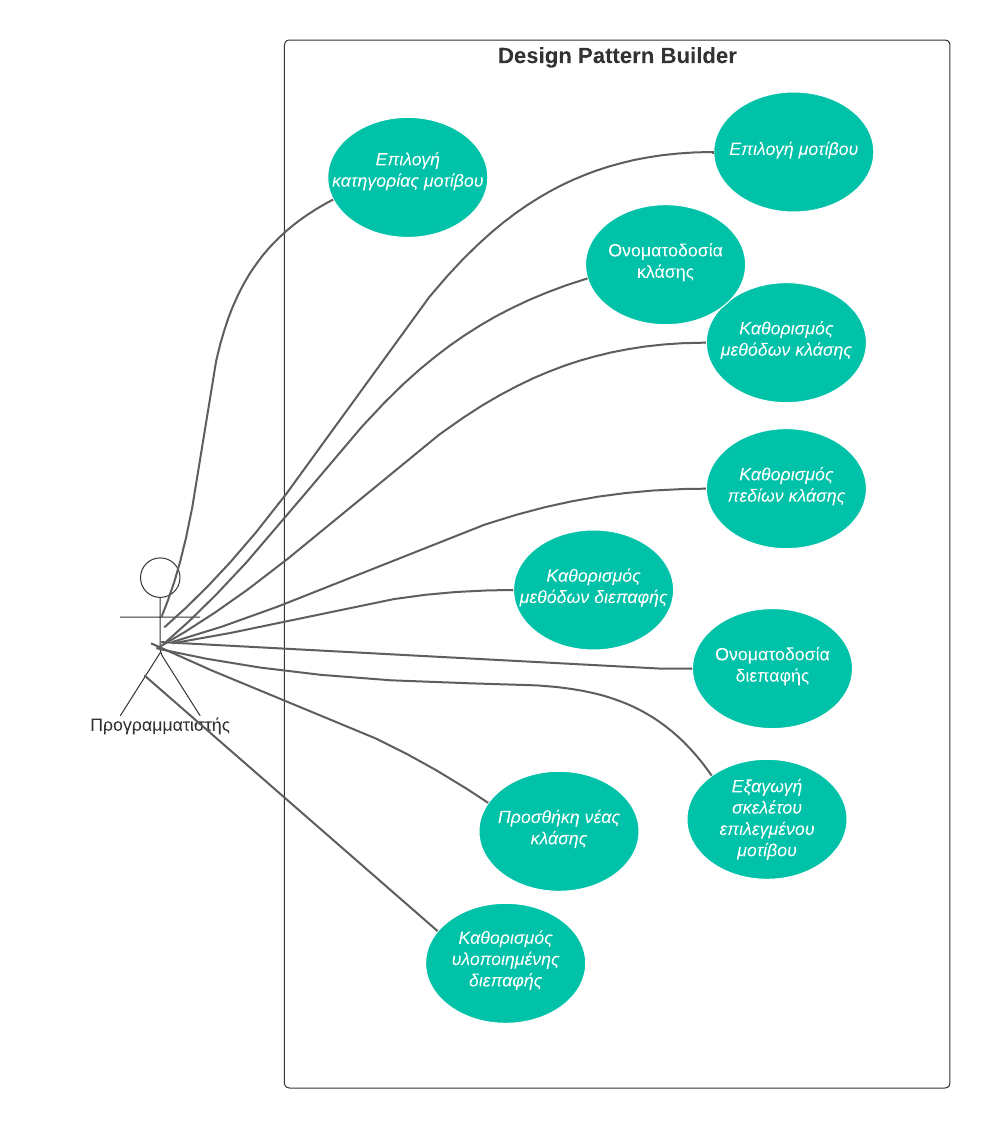
\includegraphics[width=0.65\textwidth]{Figures/use_cases.png}
	\caption{Διάγραμμα UML Περιπτώσεων Χρήστη.}
	\label{fig:useCases}
\end{figure}
\begin{table}[H]
	\hspace*{-0.2cm}
    \centering
    \scriptsize
	\begin{tabular}{|p{10cm}|}
		\hline
		\textbf{Περίπτωση χρήσης:} Επιλογή κατηγορίας μοτίβου.\\
		\hline
		\textbf{Αναγνωριστικό:} ΠΧ1\\
		\hline	
		\textbf{Προϋποθέσεις:}
		\begin{enumerate}
			\item Ο προγραμματιστής χρειάζεται να έχει επιλέξει το έργο που θα εργαστεί.
		\end{enumerate}\\
		\hline
		\textbf{Ροή γεγονότων:} \\ 
		\begin{enumerate}
			\item Η περίπτωση χρήσης ξεκινά όταν ο προγραμματιστής επιλέξει Import pattern, κάτω από το μενού pattern Genius στο παράθυρο New του eclipse. 
			\item Το σύστημα εμφανίζει έναν οδηγό.
			\item Ο προγραμματιστής επιλέγει την κατηγορία μοτίβου που επιθυμεί.
			%\item Το σύστημα εμφανίζει τα διαθέσιμα μοτίβα της κατηγορίας αυτής.
		\end{enumerate}\\
		\hline
		\textbf{Μετα-συνθήκες:} \\ Η κατάσταση του κώδικα που υλοποιεί ο προγραμματιστής παραμένει ως έχει. \\
		\hline
    \end{tabular}
    \caption{Επιλογή κατηγορίας μοτίβου.}
    \label{tab:selectPatternCategoryUC}
\end{table}
\begin{table}[H]
	\hspace*{-0.2cm}
    \centering
    \scriptsize
	\begin{tabular}{|p{10cm}|}
	\hline
		\textbf{Περίπτωση χρήσης:} Επιλογή μοτίβου \\
	\hline
		\textbf{Αναγνωριστικό:} ΠΧ2 \\
	\hline	
		\textbf{Προϋποθέσεις:} \\
		\begin{enumerate}
		 \item Ο προγραμματιστής χρειάζεται να έχει επιλέξει κατηγορία μοτίβου.
		\end{enumerate}\\
	\hline
		\textbf{Ροή γεγονότων:} \\
		\begin{enumerate}
			\item Η περίπτωση χρήσης ξεκινάει όταν ο προγραμματιστής κάνει κλικ στην πτυσσόμενη λίστα.
			\item Το σύστημα εμφανίζει τα διαθέσιμα μοτίβα.
		 	\item Ο προγραμματιστής επιλέγει το μοτίβο που επιθυμεί.
		\end{enumerate}\\
	\hline
		\textbf{Μετα-συνθήκες:} \\ Η κατάσταση του κώδικα που υλοποιεί ο προγραμματιστής παραμένει ως έχει. \\
	\hline
    \end{tabular}
    \caption{Επιλογή μοτίβου.}
    \label{tab:selectPatternUC}
\end{table}
\begin{table}[H]
	\hspace*{-0.2cm}
    \centering
    \scriptsize
	\begin{tabular}{|p{10cm}|}
	\hline
		\textbf{Περίπτωση χρήσης:} Καθορισμός μεθόδων κλάσης \\
	\hline
		\textbf{Αναγνωριστικό:} ΠΧ3 \\
	\hline	
		\textbf{Προϋποθέσεις:} \\
		\begin{enumerate}
		 \item Ο προγραμματιστής χρειάζεται να είναι στο παράθυρο επεξεργασίας της κλάσης.
		\end{enumerate} \\
	\hline
		\textbf{Ροή γεγονότων:} \\
			\begin{enumerate}
		 \item Η περίπτωση χρήσης ξεκινά όταν ο προγραμματιστής κάνει κλικ στο κουμπί Next του παραθύρου επεξεργασίας πεδίων της κλάσης.
		 \item Το σύστημα εμφανίζει ένα νέο παράθυρο με τις μεθόδους της τρέχουσας κλάσης.
		 \item Για κάθε μέθοδο:\begin{enumerate}
						 		 \item Ο προγραμματιστής επεξεργάζεται το όνομα της μεθόδου.
								 \item Ο προγραμματιστής επεξεργάζεται τον επιστρεφόμενο τύπο της μεθόδου.
		 						  \item Ο προγραμματιστής επεξεργάζεται την ορατότητα της μεθόδου.
			 		 		  \end{enumerate}
 		 \item Ο προγραμματιστής κάνει κλικ στο κουμπί finish.
 		 \item Το σύστημα κλείνει το παράθυρο.
		\end{enumerate} \\
	\hline
		\textbf{Μετα-συνθήκες:} \\
		\begin{enumerate}
			\item Το σύστημα ρυθμίζει το όνομα της κλάσης.
			\item Το σύστημα ρυθμίζει τα πεδία της κλάσης.
			\item Το σύστημα ρυθμίζει τις μεθόδους της κλάσης.
		\end{enumerate} \\
	\hline
    \end{tabular}
    \caption{Καθορισμός μεθόδων κλάσης.}
    \label{tab:setClassMethodsUC}
\end{table}
\begin{table}[H]
	\hspace*{-0.2cm}
    \centering
    \scriptsize
	\begin{tabular}{|p{10cm}|}
	\hline
		\textbf{Περίπτωση χρήσης:} Ονοματοδοσία κλάσης. \\
	\hline
		\textbf{Αναγνωριστικό:} ΠΧ4 \\
	\hline	
		\textbf{Προϋποθέσεις:} \\
		\begin{enumerate}
		 \item Ο προγραμματιστής χρειάζεται να έχει επιλέξει μοτίβο.
		\end{enumerate} \\
	\hline
		\textbf{Ροή γεγονότων:} \\
		\begin{enumerate}
		 \item Η περίπτωση χρήσης ξεκινά όταν ο προγραμματιστής κάνει κλικ στο κουμπί Next του παραθύρου επιλογής μοτίβου.
		 \item Το σύστημα εμφανίζει ένα νέο παράθυρο με τις κλάσεις και τις διεπαφές του μοτίβου.
		 \item Ο προγραμματιστής επιλέγει την κλάση που επιθυμεί.
		 \item Ο προγραμματιστής κάνει κλικ στο κουμπί edit class.
 		 \item Το σύστημα εμφανίζει ένα νέο παράθυρο όπου ο χρήστης μπορεί να επεξεργαστεί το όνομα της κλάσης.
 		 \item Ο προγραμματιστής επεξεργάζεται το όνομα της κλάσης.
 		 \item Ο προγραμματιστής κάνει κλικ στο κουμπί Next.
 		 \item Το σύστημα εμφανίζει ένα νέο παράθυρο.
		\end{enumerate} \\
	\hline
		\textbf{Μετα-συνθήκες:} \\ Η κατάσταση του κώδικα που υλοποιεί ο προγραμματιστής παραμένει ως έχει. \\
	\hline
    \end{tabular}
    \caption{Ονοματοδοσία κλάσης.}
    \label{tab:nameClassUC}
\end{table}
\begin{table}[H]
	\hspace*{-0.2cm}
    \centering
    \scriptsize
	\begin{tabular}{|p{10cm}|}
	\hline
		\textbf{Περίπτωση χρήσης:} Καθορισμός πεδίων κλάσης \\
	\hline
		\textbf{Αναγνωριστικό:} ΠΧ5 \\
	\hline	
		\textbf{Προϋποθέσεις:} \\
		\begin{enumerate}
		 \item Ο προγραμματιστής χρειάζεται να έχει επεξεργαστεί το όνομα της κλάσης
		\end{enumerate} \\
	\hline
		\textbf{Ροή γεγονότων:} \\
		\begin{enumerate}
		 \item Η περίπτωση χρήσης ξεκινά όταν ο προγραμματιστής κάνει κλικ στο κουμπί Next του παραθύρου επεξεργασίας ονόματος της κλάσης.
		 \item Το σύστημα εμφανίζει ένα νέο παράθυρο με τα πεδία της τρέχουσας κλάσης.
		 \item Για κάθε μέθοδο:\begin{enumerate}
						 		 \item Ο προγραμματιστής επεξεργάζεται το όνομα του πεδίου.
								 \item Ο προγραμματιστής επεξεργάζεται τον τύπο του πεδίου.
		 						 \item Ο προγραμματιστής επεξεργάζεται την ορατότητα του πεδίου.
			 		 		  \end{enumerate}
 		 \item Ο προγραμματιστής κάνει κλικ στο κουμπί Next.
 		 \item Το σύστημα εμφανίζει ένα νέο παράθυρο.
		\end{enumerate} \\
	\hline
		\textbf{Μετα-συνθήκες:} \\
	\hline
    \end{tabular}
    \caption{Καθορισμός πεδίων κλάσης.}
    \label{tab:setClassFieldsUC}
\end{table}
\begin{table}[H]
	\hspace*{-0.2cm}
    \centering
    \scriptsize
	\begin{tabular}{|p{10cm}|}
	\hline
		\textbf{Περίπτωση χρήσης:} Ονοματοδοσία διεπαφής  \\
	\hline
		\textbf{Αναγνωριστικό:} ΠΧ6 \\
	\hline	
		\textbf{Προϋποθέσεις:} \\
		\begin{enumerate}
		 \item Ο προγραμματιστής χρειάζεται να έχει επιλέξει μοτίβο.
		\end{enumerate} \\
	\hline
		\textbf{Ροή γεγονότων:} \\
		\begin{enumerate}
			\item Η περίπτωση χρήσης ξεκινά όταν ο προγραμματιστής κάνει κλικ στο κουμπί Next του παραθύρου επιλογής μοτίβου.
			\item Το σύστημα εμφανίζει ένα νέο παράθυρο με τις κλάσεις και τις διεπαφές του μοτίβου.
			\item Ο προγραμματιστής επιλέγει την διεπαφή που επιθυμεί.
			\item Ο προγραμματιστής κάνει κλικ στο κουμπί edit interface.
			 \item Το σύστημα εμφανίζει ένα νέο παράθυρο όπου ο χρήστης μπορεί να επεξεργαστεί το όνομα της διεπαφής.
			 \item Ο προγραμματιστής επεξεργάζεται το όνομα της διεπαφής.
			 \item Ο προγραμματιστής κάνει κλικ στο κουμπί Next.
			 \item Το σύστημα εμφανίζει ένα νέο παράθυρο.
		\end{enumerate} \\
	\hline
		\textbf{Μετα-συνθήκες:} \\
	\hline
    \end{tabular}
    \caption{Ονοματοδοσία διεπαφής.}
    \label{tab:nameInterfaceUC}
\end{table}
\begin{table}[H]
	\hspace*{-0.2cm}
    \centering
    \scriptsize
	\begin{tabular}{|p{10cm}|}
	\hline
		\textbf{Περίπτωση χρήσης:} Καθορισμός μεθόδων διεπαφής \\
	\hline
		\textbf{Αναγνωριστικό:} ΠΧ7 \\
	\hline	
		\textbf{Προϋποθέσεις:} \\
		\begin{enumerate}
			\item Η περίπτωση χρήσης ξεκινά όταν ο προγραμματιστής κάνει κλικ στο κουμπί Next του παραθύρου επεξεργασίας ονόματος της διεπαφής.
			\item Το σύστημα εμφανίζει ένα νέο παράθυρο με τις μεθόδους της τρέχουσας διεπαφής.
			\item Για κάθε μέθοδο:\begin{enumerate}
									 \item Ο προγραμματιστής επεξεργάζεται το όνομα της μεθόδου.
									\item Ο προγραμματιστής επεξεργάζεται τον επιστρεφόμενο τύπο της μεθόδου.
									  \item Ο προγραμματιστής επεξεργάζεται την ορατότητα της μεθόδου.
								   \end{enumerate}
			 \item Ο προγραμματιστής κάνει κλικ στο κουμπί finish.
			 \item Το σύστημα κλείνει το παράθυρο.
		   \end{enumerate} \\
	   \hline
		   \textbf{Μετα-συνθήκες:} \\
		   \begin{enumerate}
			   \item Το σύστημα ρυθμίζει το όνομα της διεπαφής.
			   \item Το σύστημα ρυθμίζει τις μεθόδους της διεπαφής.
		   \end{enumerate} \\
	\hline
    \end{tabular}
    \caption{Καθορισμός μεθόδων διεπαφής.}
    \label{tab:setInterfaceMethodsUC}
\end{table}
\begin{table}[H]
	\hspace*{-0.2cm}
    \centering
    \scriptsize
	\begin{tabular}{|p{10cm}|}
	\hline
		\textbf{Περίπτωση χρήσης:} Εξαγωγή σκελετού επιλεγμένου μοτίβου. \\
	\hline
		\textbf{Αναγνωριστικό:} ΠΧ8 \\ 
	\hline	
		\textbf{Προϋποθέσεις:} \\
		%TODO
		\begin{enumerate}
		 \item Ο προγραμματιστής χρειάζεται να έχει επιλέξει κατηγορία μοτίβου.
		\end{enumerate} \\
	\hline
		\textbf{Ροή γεγονότων:} \\
		\begin{enumerate}
		 \item Η Περίπτωση χρήσης ξεκινά όταν ο προγραμματιστής κάνει κλικ στο κουμπί finish στο παράθυρο επιλογής κλάσης ή διεπαφής.
		 \item Το σύστημα δημιουργεί τα απαραίτητα πηγαία αρχεία java στο επιλεγμένο πακέτο.
		 \item Το σύστημα τερματίζει.
		\end{enumerate} \\
	\hline
		\textbf{Μετα-συνθήκες:} \\ Η κατάσταση του κώδικα που υλοποιεί ο προγραμματιστής παραμένει ως έχει. \\
	\hline
    \end{tabular}
    \caption{Εξαγωγή σκελετού επιλεγμένου μοτίβου.}
    \label{tab:createPatternUC}
\end{table}
% \begin{table}[H]
% 	\hspace*{-0.2cm}
%     \centering
%     \scriptsize
% 	\begin{tabular}{|p{10cm}|}
% 	\hline
% 		\textbf{Περίπτωση χρήσης:} Ακύρωση διαδικασίας \\
% 	\hline
% 		\textbf{Αναγνωριστικό:} ΠΧ9 \\
% 	\hline	
% 		\textbf{Προϋποθέσεις:} \\
% 		%\begin{enumerate}
% 		 %\item Ο προγραμματιστής χρειάζεται να έχει επιλέξει κατηγορία μοτίβου.
% 		%\end{enumerate} \\
% 	\hline
% 		\textbf{Ροή γεγονότων:} \\
% 		\begin{enumerate}
% 		 \item Ο προγραμματιστής μπορεί ανα πάσα στιγμή να ακυρώσει την διαδικασία.
%  		 \item Το σύστημα τερματίζει τα παράθυρα.
% 		\end{enumerate} \\
% 	\hline
% 		\textbf{Μετα-συνθήκες:} \\
% 	\hline
%     \end{tabular}
%     \caption{Ακύρωση διαδικασίας.}
%     \label{tab:cancelUC}
% \end{table}
\begin{table}[H]
	\hspace*{-0.2cm}
    \centering
    \scriptsize
	\begin{tabular}{|p{10cm}|}
	\hline
		\textbf{Περίπτωση χρήσης:} Προσθήκη νέας κλάσης  \\
	\hline
		\textbf{Αναγνωριστικό:} ΠΧ10 \\
	\hline	
		\textbf{Προϋποθέσεις:} \\
		\begin{enumerate}
		 \item Ο προγραμματιστής χρειάζεται να έχει επιλέξει μοτίβο.
		 \item Το μοτίβο πρέπει να επιτρέπει την εισαγωγή καινούργιας κλάσης.
		\end{enumerate} \\
	\hline
		\textbf{Ροή γεγονότων:} \\
		\begin{enumerate}
			\item Η περίπτωση χρήσης ξεκινά όταν ο προγραμματιστής κάνει κλικ στο κουμπί Next του παραθύρου επιλογής μοτίβου.
			\item Το σύστημα εμφανίζει ένα νέο παράθυρο με τις κλάσεις και τις διεπαφές του μοτίβου.
			\item Ο προγραμματιστής Κάνει κλικ στο κουμπί Add Class.
			\item Το σύστημα προσθέτει μία νέα κλάση.
			
		\end{enumerate} \\
	\hline
		\textbf{Μετα-συνθήκες:} \\ Η κατάσταση του κώδικα που υλοποιεί ο προγραμματιστής παραμένει ως έχει. \\
	\hline
    \end{tabular}
    \caption{Προσθήκη νέας κλάσης.}
    \label{tab:addNewClass}
\end{table}
\begin{table}[H]
	\hspace*{-0.2cm}
    \centering
    \scriptsize
	\begin{tabular}{|p{10cm}|}
	\hline
		\textbf{Περίπτωση χρήσης:} Καθορισμός υλοποιημένης διεπαφής  \\
	\hline
		\textbf{Αναγνωριστικό:} ΠΧ11 \\
	\hline	
		\textbf{Προϋποθέσεις:} \\
		\begin{enumerate}
		 \item Ο προγραμματιστής χρειάζεται να έχει επιλέξει μοτίβο.
		\end{enumerate} \\
	\hline
		\textbf{Ροή γεγονότων:} \\
		\begin{enumerate}
			\item Η περίπτωση χρήσης ξεκινά όταν ο προγραμματιστής κάνει κλικ στο κουμπί Next του παραθύρου επιλογής μοτίβου.
			\item Το σύστημα εμφανίζει ένα νέο παράθυρο με τις κλάσεις και τις διεπαφές του μοτίβου.
			\item Ο προγραμματιστής επιλέγει μία κλάση που έχει προσθέσει ο ίδιος.
			\item Ο προγραμματιστής κάνει κλικ στο κουμπί edit class.
			\item Το σύστημα εμφανίζει ένα νέο παράθυρο όπου ο χρήστης μπορεί να επεξεργαστεί την διεπαφή που μπορεί να υλοποιεί η κλάση αυτή.
			\item Ο προγραμματιστής επεξεργάζεται την διεπαφή που μπορεί να υλοποιεί η κλάση αυτή.
			\item Ο προγραμματιστής κάνει κλικ στο κουμπί Next.
			\item Το σύστημα εμφανίζει ένα νέο παράθυρο.
		\end{enumerate} \\
	\hline
		\textbf{Μετα-συνθήκες:} \\ Η κατάσταση του κώδικα που υλοποιεί ο προγραμματιστής παραμένει ως έχει. \\
	\hline
    \end{tabular}
    \caption{Καθορισμός υλοποιημένης διεπαφής.}
    \label{tab:setImplementedInterface}
\end{table}
\label{sec:useCases}